\documentclass[parskip=half]{scrarticle}

\usepackage{amsmath}
\usepackage{graphicx}

\title{Lab 4: Finite State Machines}
\subtitle{CSC258H1 -- Computer Organization}

% TODO: Enter your name
\author{Your Name}

\begin{document}
\maketitle

\section*{Part I}

In this part, I encoded my states using a simple binary encoding.
Below are my schematics and timing diagram.

\begin{figure}[ht!]
    \centering
    % 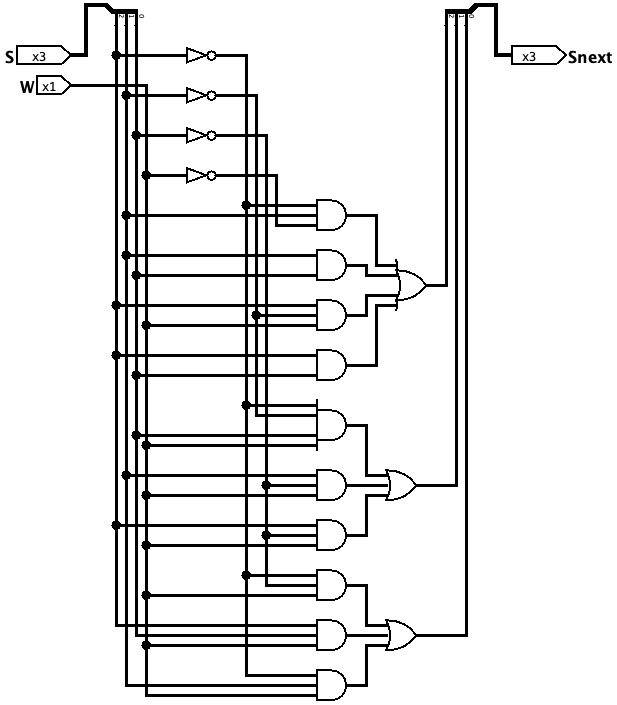
\includegraphics[width=0.3\textwidth]{lab4_part1_next_state.png}
    \caption{A schematic of Part I's NextState.}
    \label{f:part1_next_state}
\end{figure}

\begin{figure}[ht!]
    \centering
    % 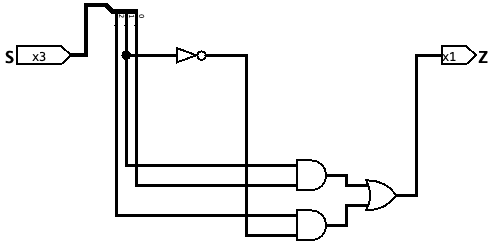
\includegraphics[width=0.5\textwidth]{lab4_part1_output.png}
    \caption{A schematic of Part I's OutputLogic.}
    \label{f:part1_output_logic}
\end{figure}

\begin{figure}[ht!]
    \centering
    % 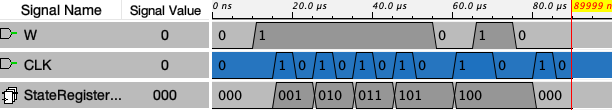
\includegraphics[width=0.5\textwidth]{lab4_part1_timing.png}
    \caption{The timing diagram for Part 1.}
    \label{f:part1_timing}
\end{figure}

\section*{Part II}

In this part, I encoded my states using a one-hot encoding.
Below are my schematics and timing diagram.

\begin{figure}[ht!]
    \centering
    % \includegraphics[width=0.3\textwidth]{lab4_part2_next_state.png}
    \caption{A schematic of Part I's NextState.}
    \label{f:part2_next_state}
\end{figure}

\begin{figure}[ht!]
    \centering
    % \includegraphics[width=0.5\textwidth]{lab4_part2_output.png}
    \caption{A schematic of Part I's OutputLogic.}
    \label{f:part2_output_logic}
\end{figure}

\begin{figure}[ht!]
    \centering
    % \includegraphics[width=0.5\textwidth]{lab4_part2_timing.png}
    \caption{The timing diagram for Part 1.}
    \label{f:part2_timing}
\end{figure}

\section*{Part III}

\begin{enumerate}
\item Propagation delay of Part I sub-circuits.
\begin{enumerate}
    \item \texttt{NextStateLogic}
    % TODO

    \item \texttt{OutputLogic}
    % TODO
\end{enumerate}

\item Propagation delay of Part II sub-circuits.
\begin{enumerate}
    \item \texttt{NextStateLogic}
    % TODO

    \item \texttt{OutputLogic}
    % TODO
\end{enumerate}

\item Compare the area of your Moore FSM using the simple binary encoding versus one-hot encoding.
    % TODO
\end{enumerate}

\end{document}